\documentclass[xetex,xcolor={table,usenames,dvipsnames}]{beamer}
\usepackage{ragged2e} % Ensure ragged2e is included
\usepackage{beamerthemesplit}
\usepackage[utf8]{inputenc}
\usepackage[T1]{fontenc}
\usepackage[english,french]{babel}
\usepackage{times}
\usepackage{tabularx}
\usepackage{dsfont}
\usepackage{textcomp}
\usepackage{amssymb}
\usepackage{graphicx}
\usepackage{bbding}
\usepackage[absolute,overlay]{textpos}
\usepackage[style=authoryear, maxbibnames=99, mincitenames=1, maxcitenames=2, backref=true, hyperref=true, dashed=false, firstinits=true, backend=bibtex, bibencoding=utf8, uniquename=false, uniquelist=false, natbib=true]{biblatex}
\renewcommand*{\bibfont}{\scriptsize}
\setbeamerfont{footnote}{size=\tiny}

% Remove quotation marks from titles
\DeclareFieldFormat[article,incollection,inproceedings,conference]{title}{#1} 

\usepackage{makecell}

\usepackage{capt-of}

\usepackage{xcolor}
\usepackage{shadowtext} 
% Define a custom color for lavender
\definecolor{lavender}{RGB}{230,230,250}
\definecolor{deepred}{RGB}{201,10,77}

\usepackage{hyperref}
 
 \hypersetup{
    colorlinks=true,      % Enable colored links
   linkcolor=violet,        % Color for internal links (sections, equations, etc.)
    citecolor=BlueViolet,      % Color for citations
    filecolor=magenta,    % Color for file links
    urlcolor=blue         % Color for URLs
}

\mode<presentation>
{
\usetheme{metropolis}


\setbeamercolor{header}{bg=MidnightBlue, fg=white} % Dark theme header
\setbeamercolor{progressdots}{fg=white} % Color for navigation dots

\setbeamertemplate{headline}{%
	% First row: Section Titles
	\begin{beamercolorbox}[wd=\paperwidth,ht=2.5ex,dp=1ex,center]{header}
		\textbf{\insertsectionnavigationhorizontal{\paperwidth}{}{}}
	\end{beamercolorbox}
	
	% Second row: Navigation Dots (one per frame under each section)
	\begin{beamercolorbox}[wd=\paperwidth,ht=1.5ex,dp=0ex,center]{progressdots}
		\hspace{5pt} % Adjust spacing
		\foreach \sec in \inserttotalsections { % Loop through sections
			\foreach \fr in {1,...,\insertsectionframe} { % Loop through frames in section
				\ifnum\fr=\insertframeinsection
				{\color{white}●} % Highlight current frame in section
				\else
				{\color{gray}○} % Other frames in section
				\fi
				\hspace{3pt} % Adjust spacing between dots
			}
			\hspace{10pt} % Space between sections
		}
	\end{beamercolorbox}
}

\setbeamertemplate{footline}{%
	\begin{beamercolorbox}[wd=\paperwidth,ht=2.5ex,dp=1ex,leftskip=3mm,rightskip=3mm]{footline}
		\hspace{3mm} \textbf{Ljudmila PETKOVI\'C} \hfill
		\textbf{\textsc{M2SOL034} : Fondamentaux de la textométrie et \texttt{TXM}} \hfill
		\textbf{\today} \hspace{3mm}
	\end{beamercolorbox}%
}

\setbeamertemplate{headline}{%
	\begin{beamercolorbox}[wd=\paperwidth,ht=2ex,dp=1ex,center]{frametitle}
		\insertsectionnavigationhorizontal{\paperwidth}{}{}
	\end{beamercolorbox}%
}
\setbeamertemplate{footline}{%
	\begin{beamercolorbox}[wd=\paperwidth,ht=4ex,dp=1ex,leftskip=3mm,rightskip=3mm]{footline}
		\hspace{3mm} 
		\textcolor{gray}{\textbf{Ljudmila PETKOVI\'C}} \hfill
		\textcolor{gray}{\textbf{\textsc{M2SOL034} : Fondamentaux de la textométrie et \texttt{TXM}}} \hfill 
		\textcolor{gray}{\textbf{\today}} \hspace{3mm}
		\textcolor{gray}{\textbf{\insertframenumber{} / \inserttotalframenumber}} \hspace{3mm} % Page number in bottom-right
	\end{beamercolorbox}%
	
	% Add the logo only if we're NOT on the title slide
	\ifnum\insertframenumber>0
	\begin{textblock*}{2.5cm}(\paperwidth-2cm,1\textheight) % Move slightly down and right
		
\includegraphics[width=1.2cm]{img/logo.png} % Adjusted logo size
	\end{textblock*}
	\fi
}









%\usecolortheme{beaver}
\usefonttheme{professionalfonts}
}







\usepackage{listings}

\lstset{ 
  language=C,                     % Set language
  basicstyle=\ttfamily\small,      % Set basic style to small monospaced font
  keywordstyle=\color{blue},       % Set keywords in blue
  commentstyle=\color{gray},       % Set comments in gray
  stringstyle=\color{red},         % Set strings in red
  numbers=left,                    % Line numbers on the left
  numberstyle=\tiny\color{gray},   % Style for line numbers
  stepnumber=1,                    % Line number step
  showstringspaces=false,          % Don't show spaces in strings
  tabsize=4,                       % Set tab size
  breaklines=true,                 % Break long lines
  captionpos=b                     % Caption position bottom
}

\usepackage[font=scriptsize,justification=centering]{caption}
\setbeamercolor{normal text}{fg=black,bg=black}
\setbeamercolor{frametitle}{fg=purple,bg=white}
\setbeamercolor{background canvas}{bg=white}
\setbeamercolor{title}{fg=purple}
\setbeamercolor{subtitle}{fg=purple}
\setbeamercolor{section in toc}{fg=purple}
\setbeamercolor{footline}{fg=purple,bg=white}
%\setbeamercolor{block title}{fg=purple,bg=white}
%\setbeamercolor{block body}{fg=white,bg=black}

\newcommand{\bolder}[1]{{\color{purple}\bfseries#1}}

% Set bullet points color to gold
\setbeamercolor{itemize item}{fg=violet}
\setbeamercolor{itemize subitem}{fg=violet}
\setbeamercolor{itemize subsubitem}{fg=violet}


\beamertemplatetransparentcovered
\beamerboxesdeclarecolorscheme{myalert}{red}{black!5!averagebackgroundcolor}
\beamerboxesdeclarecolorscheme{mybox}{blue}{black!5!averagebackgroundcolor}


%% Customize the colors for the footer
%\setbeamercolor{footline}{bg=white,fg=violet} % Set background to violet and text to white
%\setbeamercolor{footline title}{bg=white,fg=violet}
%\setbeamercolor{footline section}{bg=white,fg=violet}
%\setbeamercolor{footline page}{bg=white,fg=violet}
%
%% Customize the footer
%\setbeamertemplate{footline}{%
%  \leavevmode%
%  \hbox{%
%    \begin{beamercolorbox}[wd=.333\paperwidth,ht=2.25ex,dp=1ex,leftskip=3mm,rightskip=3mm,center]{footline title}%
%      \usebeamerfont{author in head/foot}\insertshorttitle
%    \end{beamercolorbox}%
%    \begin{beamercolorbox}[wd=.333\paperwidth,ht=2.25ex,dp=1ex,center]{footline section}%
%      \usebeamerfont{author in head/foot}\insertsection
%    \end{beamercolorbox}%
%    \begin{beamercolorbox}[wd=.333\paperwidth,ht=2.25ex,dp=1ex,right,center]{footline page}%
%      \usebeamerfont{author in head/foot}\insertframenumber{} / \inserttotalframenumber
%    \end{beamercolorbox}%
%  }%
%  \vskip0pt%
%}

\setbeamercolor{block title}{bg=violet,fg=white}
\setbeamercolor{block body}{bg=lavender,fg=black}


 \newcommand{\cf}{\textit{cf.} }
 \newcommand{\ie}{\textit{i.e.} }
 \newcommand{\ev}{espace vectoriel }
 \newcommand{\ssi}{si et seulement si }




\newcommand{\espc}[1]{\esp\left[ #1 \right]}

\newcommand{\defe}{\stackrel{\mbox{\begin{tiny}
 déf
 \end{tiny}}}{=}}
 \newcommand{\tend}[2]{\mathop{\longrightarrow}\limits_{#1\rightarrow #2}}

\newcommand{\rem}{\noindent\textbf{Remark : }}
\newcommand{\rems}{\textbf{Remarques: }}

\newcommand{\exs}{\textbf{Exemples: }}

\newcommand{\imp}[1]{\textbf{\textit{#1}}}


%\newtheorem{lem}{\textbf{Lemma}} 
%\newtheorem{theo}{\textbf{Theorem}} %[section]
%\newtheorem{prop}{\textbf{Proposition}}%[chapter]
%\newtheorem{coro}{\textbf{Corollary}}%[chapter]
%\newtheorem{hyp}{\textbf{Hypothesis}}
%\newtheorem{defi}{\textbf{Definition}}
%\newtheorem{pdefi}{\textbf{Proposition-D\'{e}finition}}

%\newenvironment{proof}[1][Proof : ]{\begin{trivlist}
%\item[\hskip \labelsep {\bfseries #1}]}{\hfill $\Box$\end{trivlist}}
%
%\newtheorem{lem}{\textbf{Lemme}} 
%\newtheorem{theo}{\textbf{Théorème}} %[section]
%\newtheorem{prop}{\textbf{Proposition}}%[chapter]
%\newtheorem{coro}{\textbf{Corollaire}}%[chapter]
%\newtheorem{hyp}{\textbf{Hypothèses}}
%\newtheorem{defi}{\textbf{Définition}}
%\newtheorem{pdefi}{\textbf{Proposition-D\'{e}finition}}
%\newtheorem{rmq}{\textbf{Remarque}} 

\usepackage{pgf,pgfarrows,pgfnodes,pgfautomata,pgfheaps,pgfshade}


%\font\bbfnt=msbm6
%\def\bbN{\mbox{\bbfnt N}}
%\def\bbR{\mbox{\bbfnt R}}
%\title{Champs aléatoires gaussiens}
%\author{Victor Rabiet}
%\institute{EMSE}
%\date[APSSE]{Présentation du 17 décembre 2015}

%===================================================
%===================================================
\usepackage{etoolbox} % Required for \apptocmd

% Make subitems smaller
\makeatletter
\patchcmd{\itemize}
{\def\makelabel}
{\setlength{\itemsep}{2pt} % Adjust spacing if needed
	\def\makelabel{\textbf{\scriptsize}}} % Change to \small, \footnotesize, or \scriptsize
{}
{}
\makeatother

% Make subsubitems even smaller
\makeatletter
\patchcmd{\itemize}
{\def\makelabel}
{\setlength{\itemsep}{1pt} % Adjust spacing
	\def\makelabel{\textbf{\tiny}}} % Use a smaller font size
{}
{}
\makeatother

% Change subitem bullets to circles
\setbeamertemplate{itemize subitem}{\raisebox{0.15em}{\scriptsize$\circ$}}

% Optionally, change subsubitem bullets to smaller circles
\setbeamertemplate{itemize subsubitem}{\raisebox{0.15em}{\tiny$\circ$}}


\addtobeamertemplate{frametitle}{}{%
\begin{textblock*}{2cm}(11.5cm,0.2cm) % Adjust position here

\end{textblock*}}


\addbibresource{bibliographie.bib}


\let\oldnocite\nocite
\makeatletter
\renewcommand*{\nocite}[1]{\oldnocite{#1}\Hy@backout{#1}}
\makeatother

\renewcommand*{\bibfont}{\footnotesize}

\DeclareCiteCommand{\cite}
{\usebibmacro{prenote}}
{\usebibmacro{citeindex}%
	\printtext[bibhyperref]{\usebibmacro{cite}}}
{\multicitedelim}
{\usebibmacro{postnote}}

\DeclareCiteCommand*{\cite}
{\usebibmacro{prenote}}
{\usebibmacro{citeindex}%
	\printtext[bibhyperref]{\usebibmacro{citeyear}}}
{\multicitedelim}
{\usebibmacro{postnote}}

\DeclareCiteCommand{\parencite}[\mkbibparens]
{\usebibmacro{prenote}}
{\usebibmacro{citeindex}%
	\printtext[bibhyperref]{\usebibmacro{cite}}}
{\multicitedelim}
{\usebibmacro{postnote}}

\DeclareCiteCommand*{\parencite}[\mkbibparens]
{\usebibmacro{prenote}}
{\usebibmacro{citeindex}%
	\printtext[bibhyperref]{\usebibmacro{citeyear}}}
{\multicitedelim}
{\usebibmacro{postnote}}

\DeclareCiteCommand{\footcite}[\mkbibfootnote]
{\usebibmacro{prenote}}
{\usebibmacro{citeindex}%
	\printtext[bibhyperref]{ \usebibmacro{cite}}}
{\multicitedelim}
{\usebibmacro{postnote}}

\DeclareCiteCommand{\footcitetext}[\mkbibfootnotetext]
{\usebibmacro{prenote}}
{\usebibmacro{citeindex}%
	\printtext[bibhyperref]{\usebibmacro{cite}}}
{\multicitedelim}
{\usebibmacro{postnote}}

%\DeclareCiteCommand{\textcite}
%  {\boolfalse{cbx:parens}}
%  {\usebibmacro{citeindex}%
	%   \printtext[bibhyperref]{\usebibmacro{textcite}}}
%  {\ifbool{cbx:parens}
	%     {\bibcloseparen\global\boolfalse{cbx:parens}}
	%     {}%
	%   \multicitedelim}
%  {\usebibmacro{textcite:postnote}}

%\DeclareCiteCommand{\textcite}
%{\usebibmacro{cite:init}%
%	\usebibmacro{prenote}}
%{\usebibmacro{citeindex}%
%	\printtext[bibhyperref]{\usebibmacro{textcite}}}
%{}
%{\printtext[bibhyperref]{\usebibmacro{textcite:postnote}}%
%	\usebibmacro{cite:post}}

%\DeclareCiteCommand{\textcite}
%{\usebibmacro{prenote}}
%{\printnames[final={\&}]{author} \bibhyperref{(\printfield{year})}}
%{\multicitedelim}
%{\usebibmacro{postnote}}




	
\DefineBibliographyStrings{french}{%
	backrefpage = {voir p\adddot},%
	backrefpages = {voir pp\adddot}%
}
\DeclareFieldFormat{pagerefformat}{\mkbibparens{{\color{red}\mkbibemph{#1}}}}
\renewbibmacro*{pageref}{%
	\iflistundef{pageref}
	{}
	{\printtext[pagerefformat]{%
			\ifnumgreater{\value{pageref}}{1}
			{\bibstring{backrefpages}\ppspace}
			{\bibstring{backrefpage}\ppspace}%
			\printlist[pageref][-\value{listtotal}]{pageref}}}}


\begin{document}


\title{{\large Corpus, ressources et linguistique outillée $\cdot$ \textsc{M2SOL034}}}
\subtitle{CM 2 : Fondamentaux de la textométrie et \texttt{TXM}}
\author{\footnotesize{Ljudmila PETKOVI\'C}}
\institute{{\scriptsize Sorbonne Université\\Master \og{}Langue et Informatique\fg{} (\textsc{M1} ScLan)\\\textsc{UFR} Sociologie et Informatique pour les Sciences Humaines}\\~\\{\tiny Cours adapté de \textcite{fort}, \textcite{lejeune2023} et \textcite{pincemin2008}}}
\date{\scriptsize{Semestre 2, 2024-2025\\\today}}



	\frame{\titlepage}

\section{Les \og{}métries\fg{}}


\begin{frame}{De la lexicométrie à la textométrie}
	\begin{block}{Analyse de données textuelles (\textsc{ADT})}
		\justifying Application de calculs sur des données textuelles (grands corpus).
	\end{block}
	Développement des disciplines en France :
	\begin{itemize}
		\item \bolder{lexico}métrie (\textit{circa} 1970) : application sur le lexique (mots)
		\begin{itemize}
			\item statistique lexicale : évaluation de la richesse du vocabulaire
			\item analyses factorielles, classifications : cartographies synthétiques
		\end{itemize}
		\item \bolder{texto}métrie (\textit{circa} 2004) : application sur le texte
		\item \bolder{logo}métrie (\textit{circa} 2004) : application sur le discours
	\end{itemize}
\end{frame}

\begin{frame}{Communautés scientifiques concernées}
	Sciences humaines et sociales :
	\begin{itemize}
		\item corpus scientifiques
		\item archives historiques
		\item dépouillement d'enquêtes avec questions ouvertes
		\item \oe{}uvres littéraires
		\item $\dots$
	\end{itemize}
\end{frame}

\begin{frame}{Enjeux textométriques}
	Développer des modèles statistiques pour rendre compte de caractéristiques significatives des données textuelles :
	\begin{itemize}
		\item attirances contextuelles des mots 
		\begin{itemize}
			\item phraséologie, champs thématiques$\dots$
		\end{itemize}
		\item linéarité et organisation interne du texte
		\begin{itemize}
			\item mots répartis au fil du texte ou apparaissant en \og{}rafales\fg{}
		\end{itemize}
		\item contrastes intertextuels 
		\begin{itemize}
			\item mesure statistique du sur-/sous-emploi d’un mot dans un texte
			\item repérage des mots et des phrases caractéristiques d’un texte
		\end{itemize}
		\item indicateurs d’évolution lexicale 
		\begin{itemize}
			\item période caractéristique d’un terme
			\item détection des ruptures significative
		\end{itemize}
	\end{itemize} 
\end{frame}

\begin{frame}{La textométrie au service de la linguistique outillée}
	
	
	
Calculs mathématiquement et \textbf{linguistiquement} significatifs :\\
{\small$\neq$ recherche d'information : focus sur les problématiques documentaires}
	\begin{itemize}
		\item  probabilités, statistiques, analyse des données
		\item expression et traduction mathématique d'hypothèses sur la langue et la textualité
		\item vue globale \textit{vs.} consultation ciblée des contextes d'emploi
	\end{itemize}
	
Retour au texte : prendre du recul pour interpréter des résultats.\\
\og{}\textit{L'outil dégrossit, l'humain interprète}\fg{} \citep{lejeune2023}\\
{\small$\neq$ analyse sémantique latente : passage à d'autres disciplines}\\
{\small$\neq$ \textsc{TAL} : calibrage des calculs}
\end{frame}

\begin{frame}{Modèle \textsc{SÉMA}}
	\bolder{S}ynthèse : calculs statistiques $\rightarrow$ vues synthétiques significatives
	\begin{itemize}
		\item caractérisation des singularités d'un texte
		\item repérage des thèmes
	\end{itemize}
	
	\bolder{É}dition : présentation du texte (accès aux contextes)
	
	\bolder{M}oteur de recherche : repérage des occurrences d'un motif donné
	
	\bolder{A}nnotation : enrichissement des corpus au fil des analyses
\end{frame}

\begin{frame}{Au-delà des moteurs d'internet}
	Mettre en évidence des contrastes significatifs
	\begin{itemize}
	\item caractérisation et repérage des singularités
\end{itemize}	
	Expliciter les fonctionnalités à tous les niveaux 
	\begin{itemize}
		\item théoriques, informatiques, méthodologiques$\dots$
	\end{itemize}
Vision globale, qualitative, respectant une pluralité de réponses
	\medskip
	
	{\small $\neq$ moteurs d'internet
		\begin{itemize}
			\item plus une page est citée, plus elle est mise en valeur
			\item critères de sélection opaques $\approx$ \og{}boîtes noires\fg{}
			\item conception \og{}compétitive\fg{} : résultats classés par ordre de pertinence
		\end{itemize}}
	

\end{frame}

\section{(Ré)introduction à \texttt{TXM}}

\begin{frame}{\texttt{TXM}\footnote{\url{https://txm.gitpages.huma-num.fr/textometrie/}}}
\begin{itemize}
	\item projet \textsc{ANR} \og{}Textométrie\fg{}
	\item communauté d'utilisateurs et de développeurs active
	\item logiciel libre : pérénité $\rightarrow$ possibilité de faire évoluer le code
	\item multi-plateforme (Windows, Mac, Linux)
	\item portail en ligne \texttt{txm-demo}\footnote{\url{https://txm-demo.huma-num.fr/txm/}}
	\item technologies de corpus supportées
	\begin{itemize}
		\item Unicode, \textsc{XML}, \textsc{TEI}, outils de \textsc{TAL}, \textsc{CQP}, \textsc{R}
		\end{itemize}
	\item analyse de grands corpus, structurés ou non
	\item intégration des outils externes 
	\begin{itemize}
		\item p. ex. \texttt{TreeTagger}\footnote{\url{https://www.cis.uni-muenchen.de/~schmid/tools/TreeTagger/}} -- étiquetage morphosyntaxique
		\end{itemize}
\end{itemize}
\end{frame}

\begin{frame}{Avantages de l'utilisation de \texttt{TXM}}
	\begin{itemize}
		\item \textbf{interface} très complète
		\item \textbf{robustesse} : permet de traiter jusqu'à 10 millions de mots
		\item \textbf{puissance} : permet d'intégrer toutes sortes de traitement via le logiciel \textsc{R} (de
		statistiques)
		\item \textbf{rapidité} : permet d'interroger des millions de mots très efficacement via \textsc{CQP}
		(\textit{Corpus Query Processor})
	\end{itemize}
	\begin{flushright}
		{\small\citep{fort}}
	\end{flushright}
	
\end{frame}
\begin{frame}{Fonctionnalités}
	\bolder{Analyses statistiques basiques}
	\begin{itemize}
		\item Index
		\item Concordances
		\item Cooccurrences
	\end{itemize}
	\bolder{Analyses avancées}
		\begin{itemize}
		\item Attirance contextuelle des mots et des expressions
		\item Spécificités lexicales
		\item Linéarité et organisation interne du texte
		\item Comparaisons de sous-corpus
	\end{itemize}
	

\end{frame}

\begin{frame}{Lexique}
	\begin{itemize}
		\item liste de formes (ou de tokens)
		\item fréquence d'apparition
		\item lemmatisation / étiquetage (\texttt{TreeTagger})
		\begin{itemize}
			\item \textcolor{deepred}{tâches maîtrisées mais non résolues}
			\item forme canonique (suppose corpus monolingue pour \texttt{TXM})
			\item étiquettes p. ex. \texttt{NOM, ADJ, VER, ADV} + morphologie
		\end{itemize}
		\item revisiter le mot dans son contexte
		\item allers et retours entre le lexique et le corpus
	\end{itemize}
\end{frame}

\begin{frame}{Concordances}
	Vue synthétique des occurrences d'une forme (d'un motif) :
	\begin{itemize}
		\item ses contextes d'apparition
		\item triés de différentes façons
	\end{itemize}
	
	Utilisations :
	\begin{itemize}
		\item distribution dans le corpus
		\item expressions dérivées
		\item structures grammaticales
	\end{itemize}
	
	
\end{frame}

\begin{frame}{Concordances}
	\begin{block}{Concordancier}
		\justifying
		Logiciel qui permet de faire un tri rapide de tous les mots d'un texte (ou d'un ensemble de textes), de situer des mots-pivot en contexte (\textsc{KWIC} – \textit{Key Word in Context}), de compter le nombre d'occurrences, etc., à partir de chaînes de caractères.
	\end{block}
	\begin{figure}[h] % Use [H] to force the figure to stay in place
		\centering
		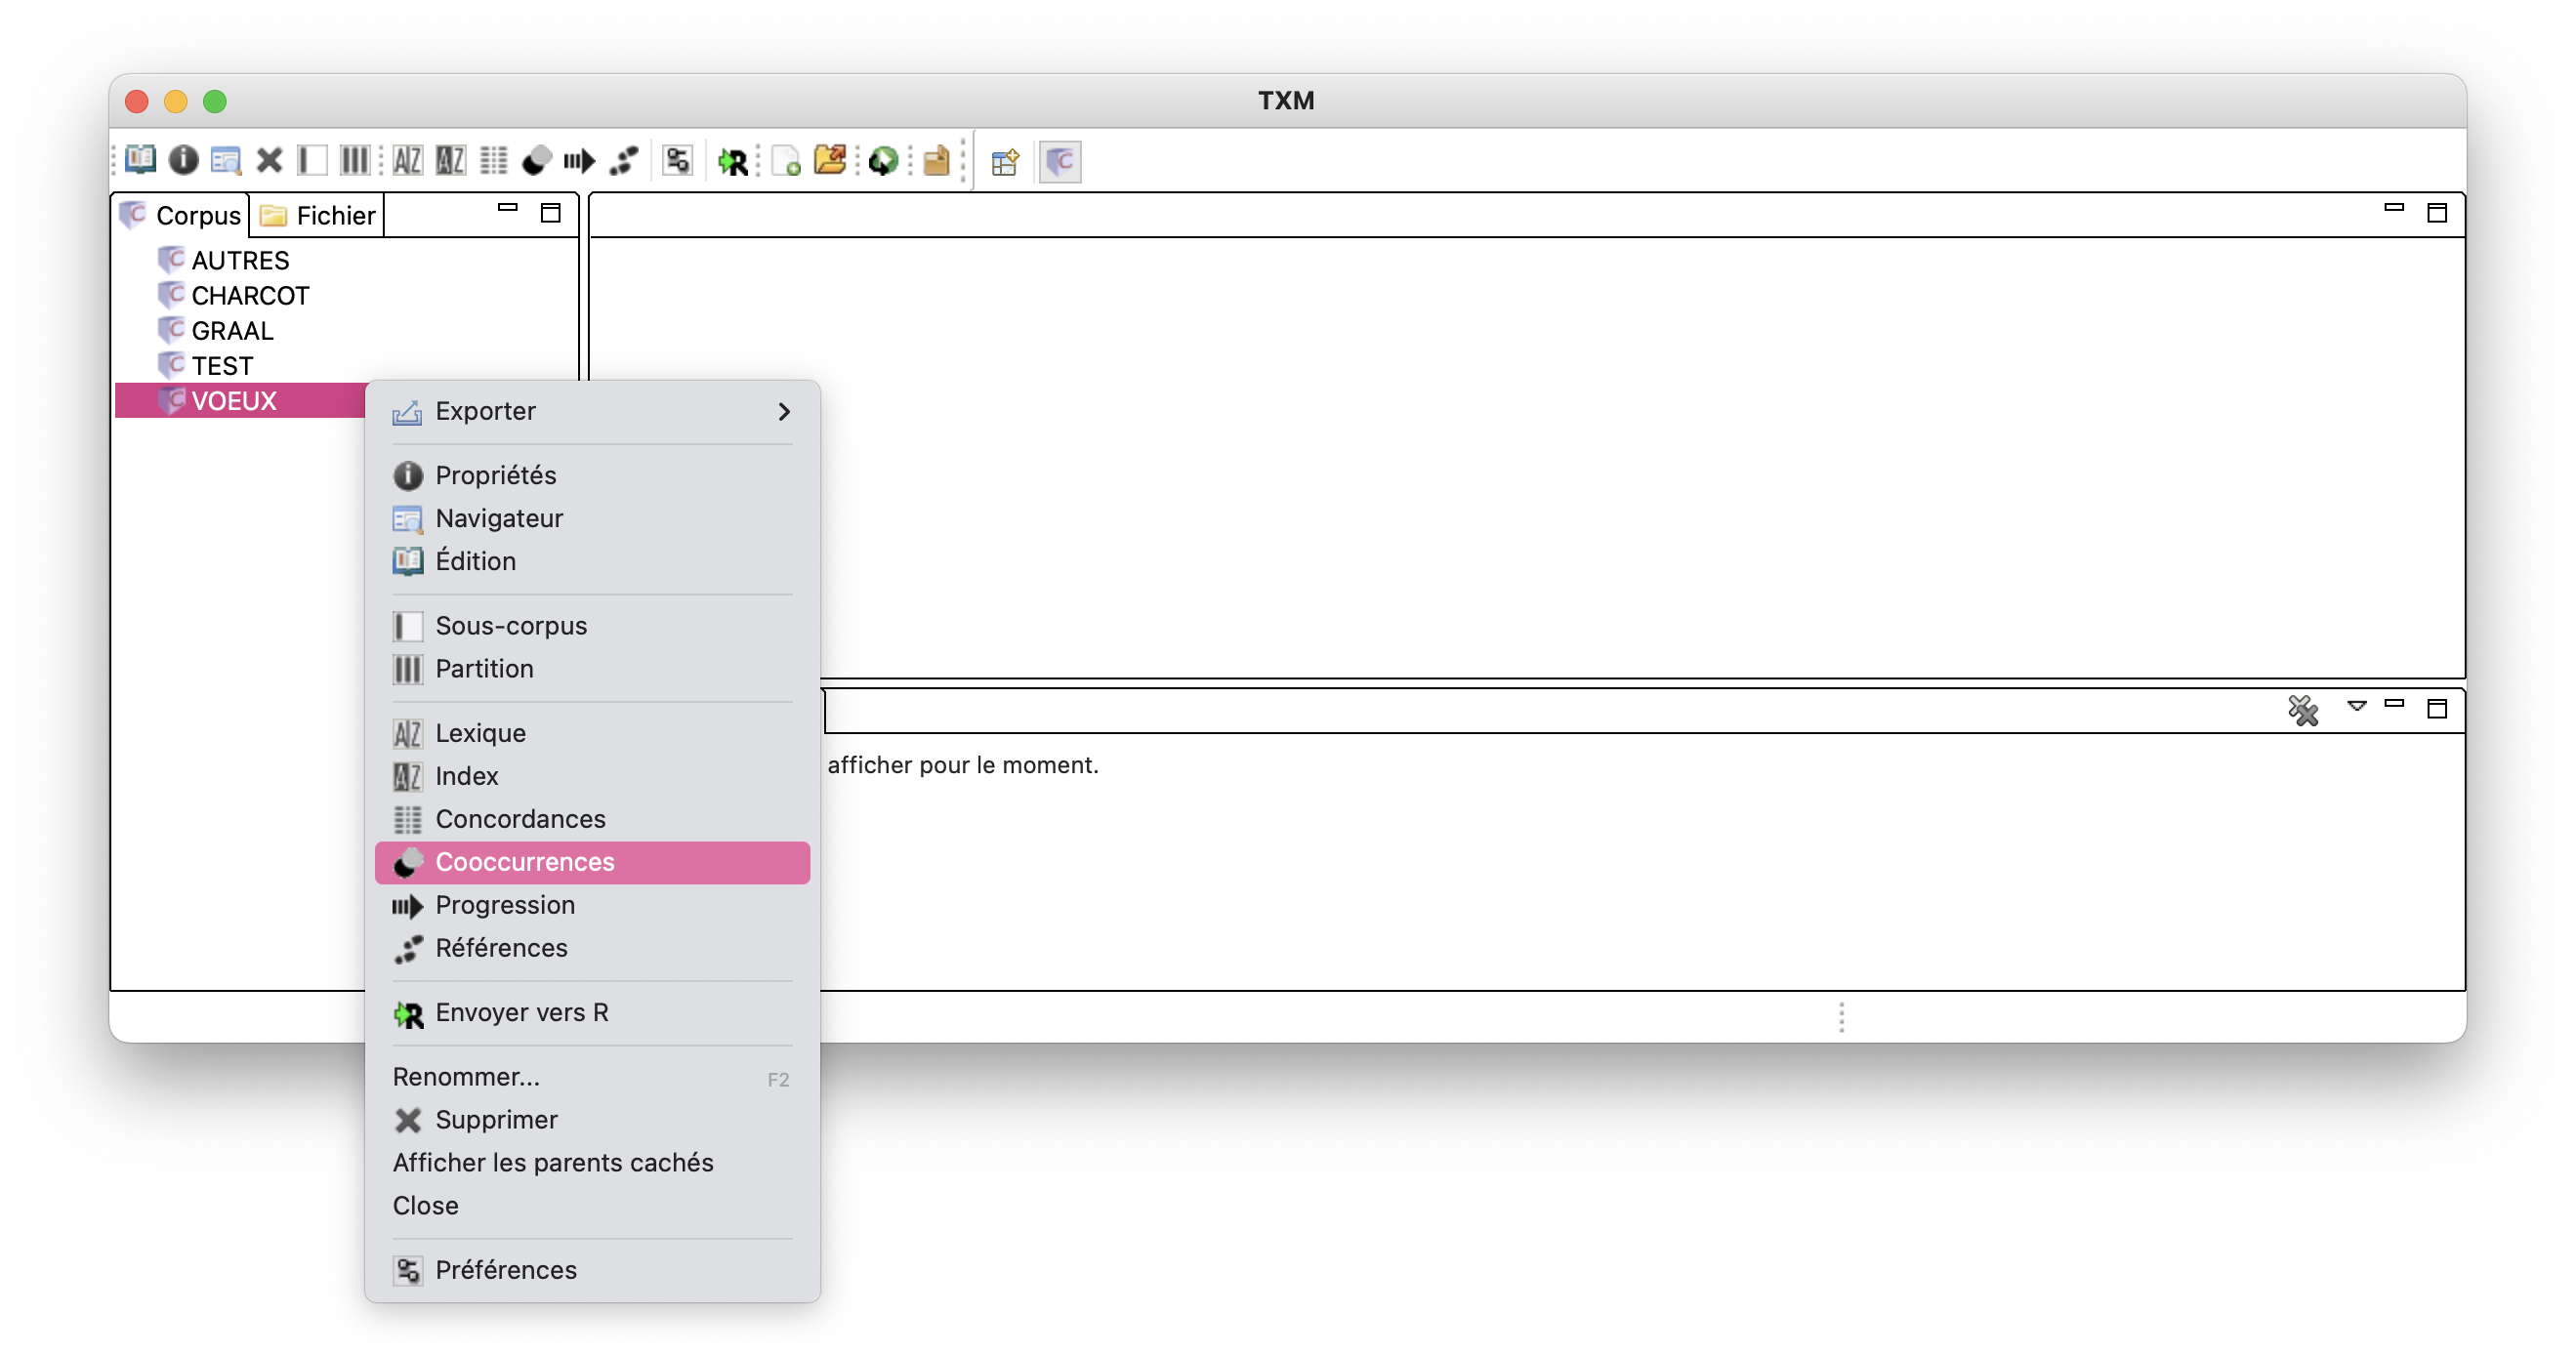
\includegraphics[width=0.80\linewidth]{img/concordances.png}
		\caption{Accès au concordancier.}
		\label{fig:ling_out_TAL}
	\end{figure}
\end{frame}

\begin{frame}{Concordances}
		\begin{figure}[h] % Use [H] to force the figure to stay in place
		\centering
		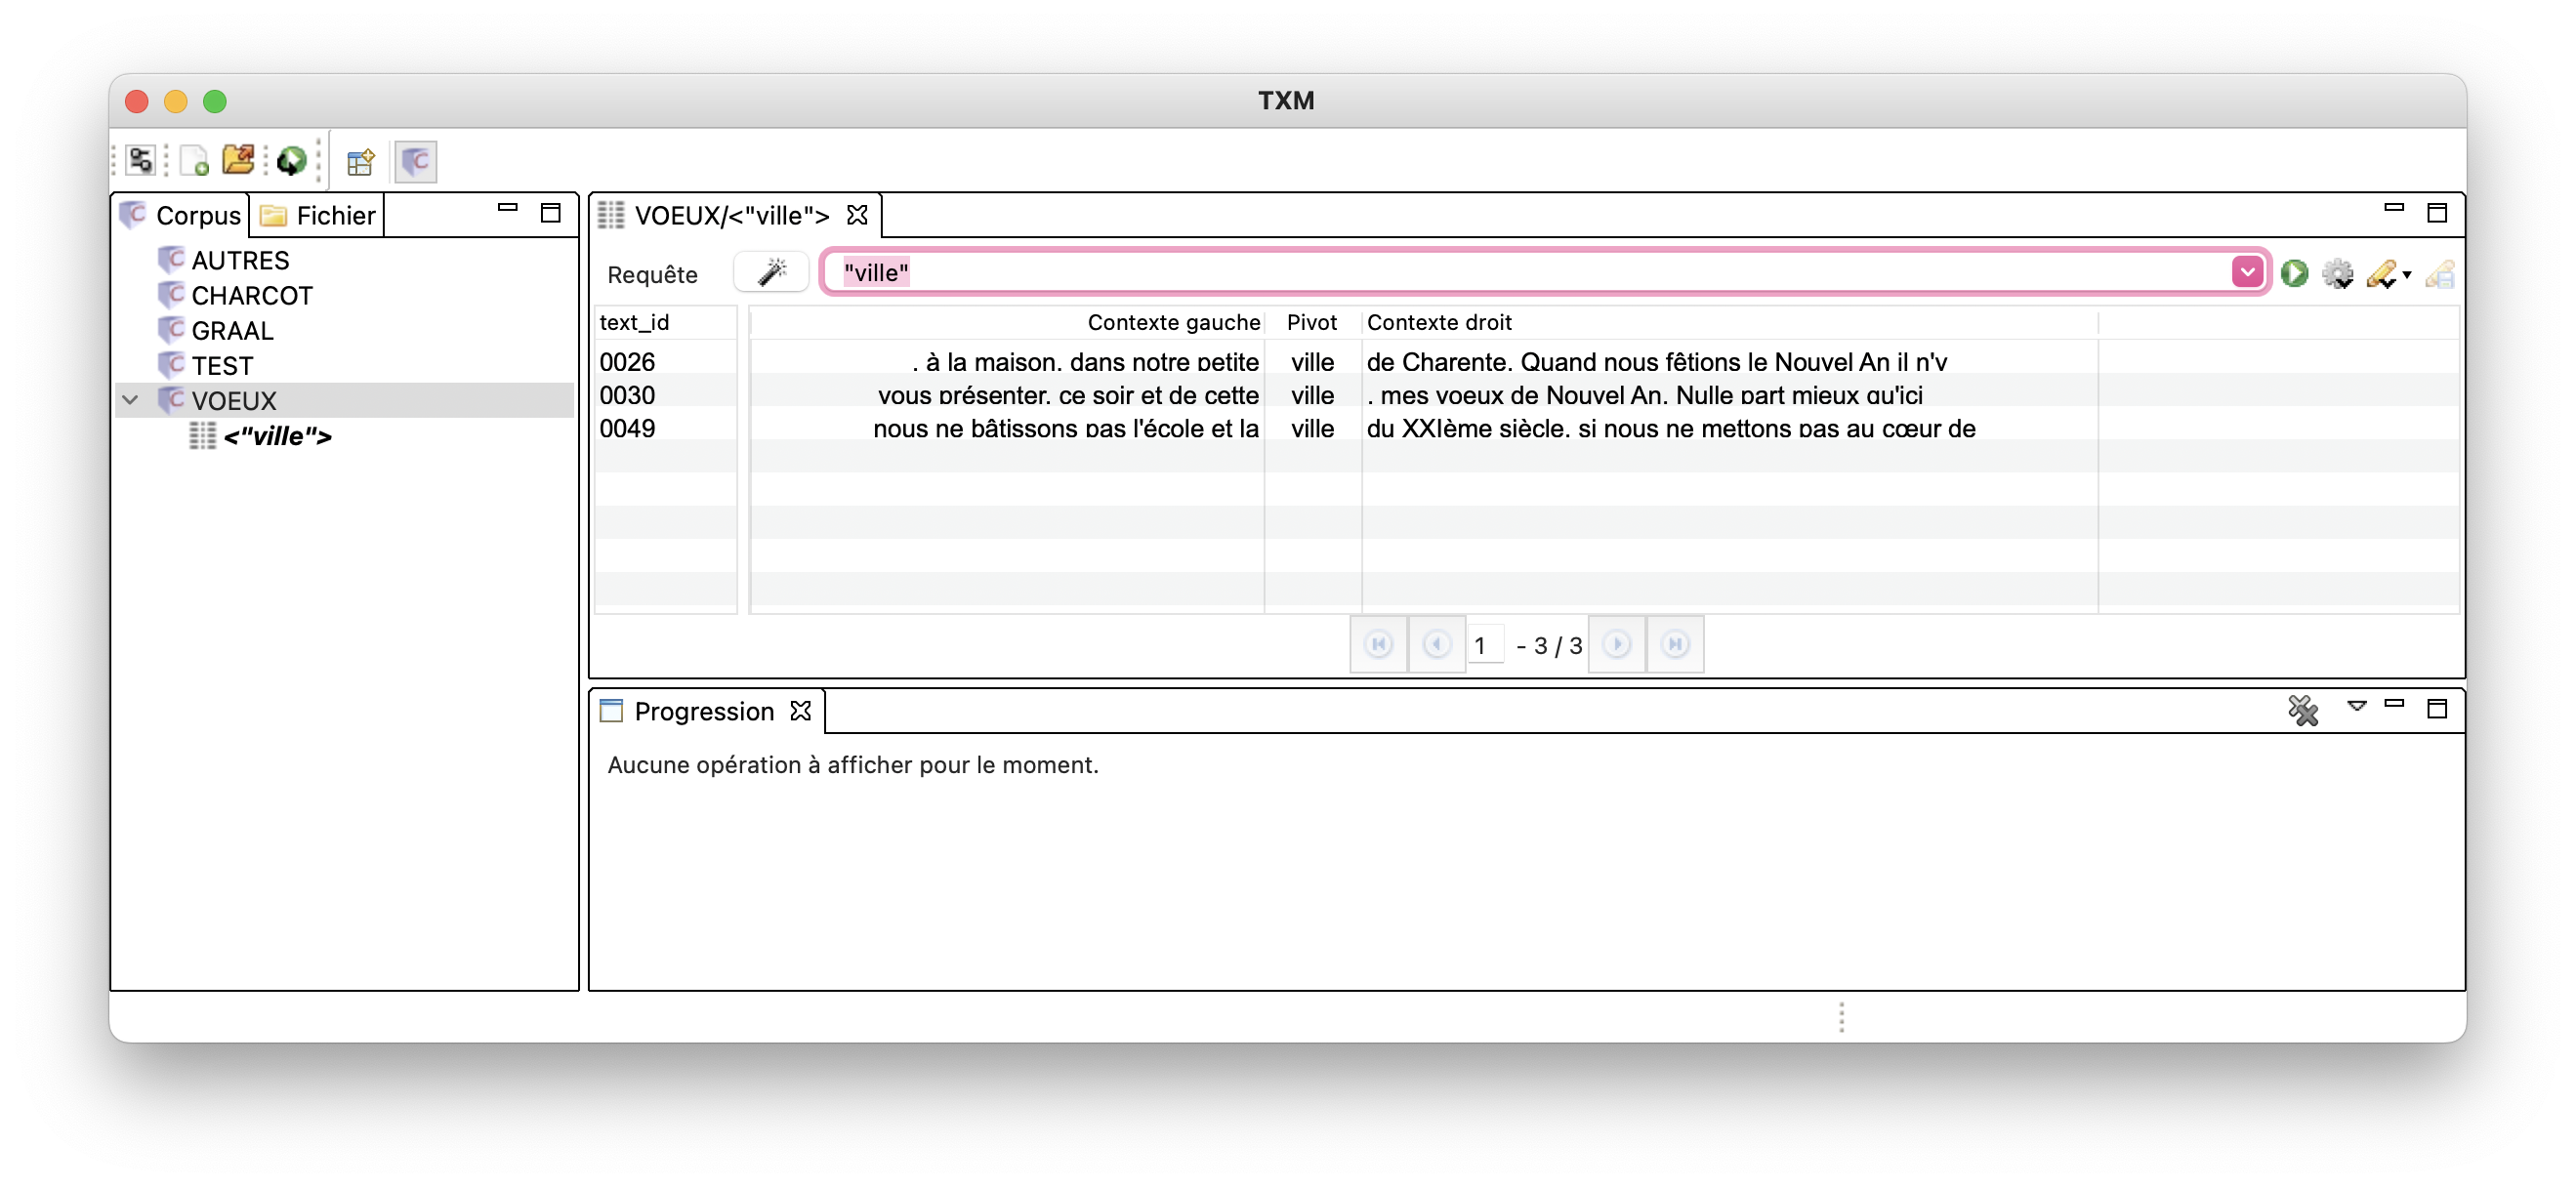
\includegraphics[width=1\linewidth]{img/ville.png}
		\caption{Affichage du mot-pivot \og{}ville\fg{} dans le corpus \texttt{VOEUX}.}
		\label{fig:ling_out_TAL}
	\end{figure}
\end{frame}

\begin{frame}{Concordances : le pivot}
Le pivot peut être :
\begin{itemize}
	\item un mot (cas le plus simple)
	\item une séquence de mots
	\item un motif simple (détectable avec une expression régulière)
	\item un motif complexe (lexico-)syntaxique en langage \textsc{CQL} (\textit{Corpus Query Language})
\end{itemize}

\end{frame}

\begin{frame}{Propriétés du pivot}
	\begin{figure}[h] % Use [H] to force the figure to stay in place
		\centering
		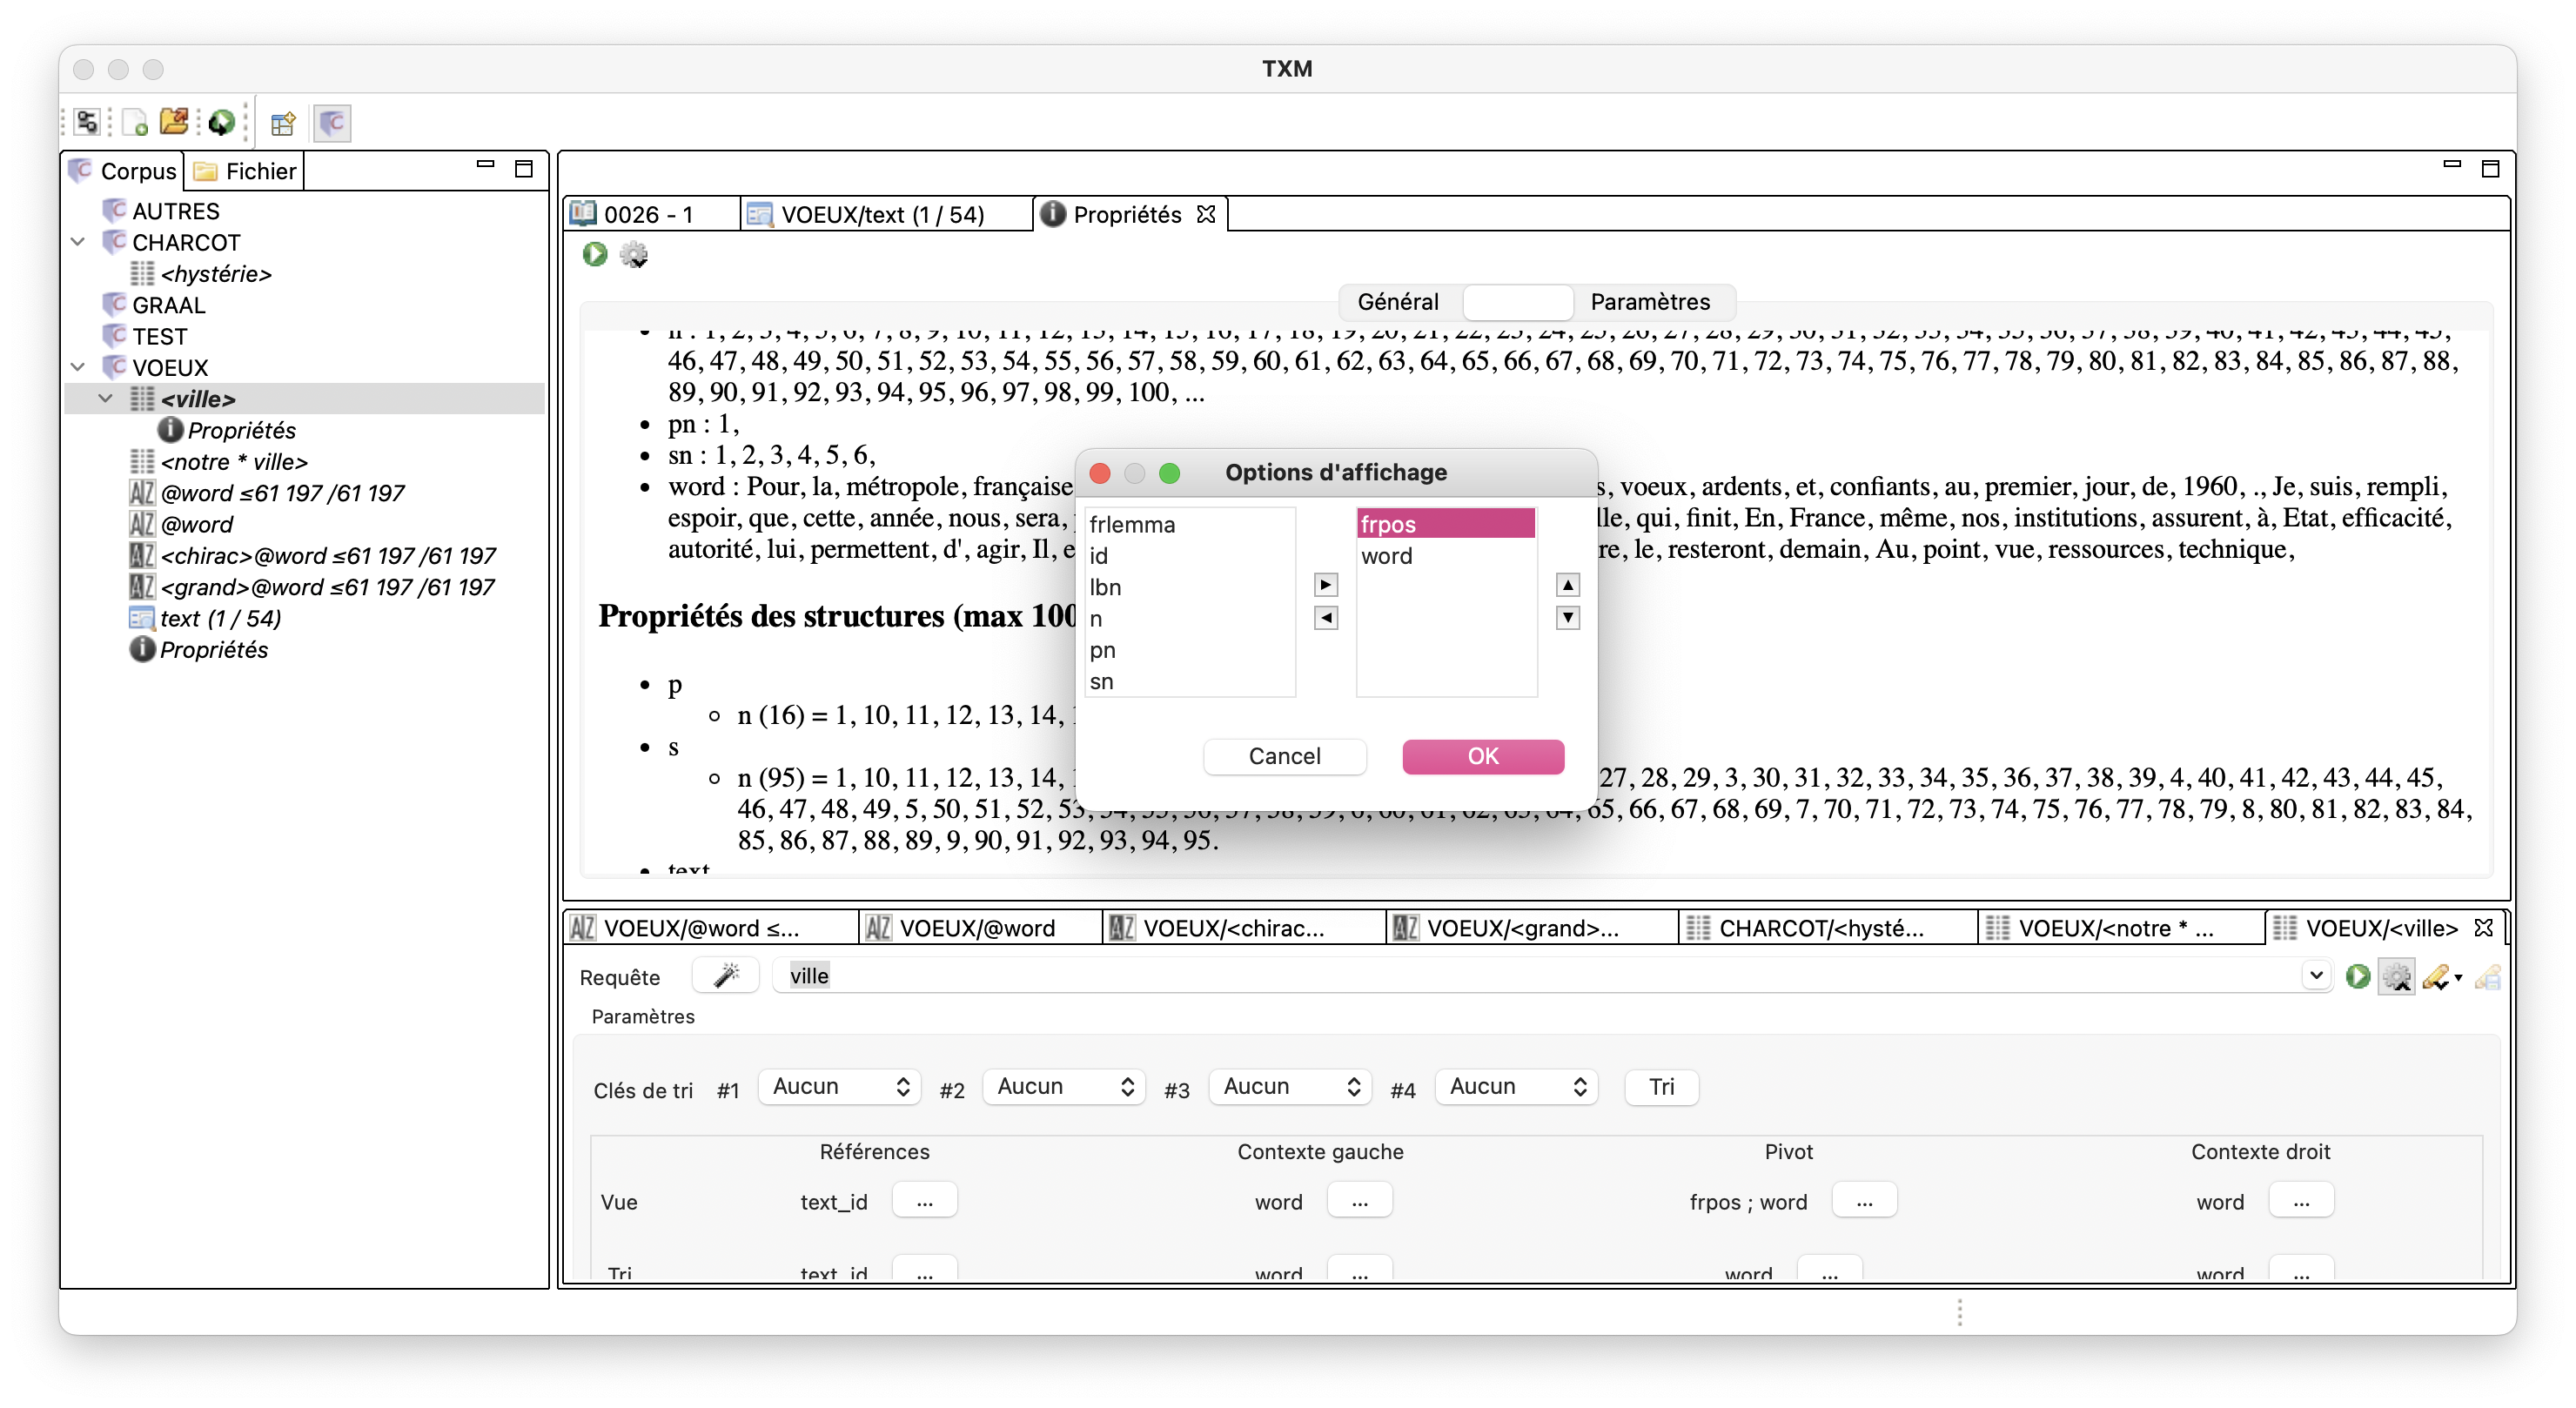
\includegraphics[width=1\linewidth]{img/proprietes_pivot.png}
		\caption{Propriétés du pivot \og{}ville\fg{} dans le corpus \texttt{VOEUX}.}
		\label{fig:ling_out_TAL}
	\end{figure}
\end{frame}

\begin{frame}{Propriétés du pivot}
			\begin{figure}[h] % Use [H] to force the figure to stay in place
		\centering
		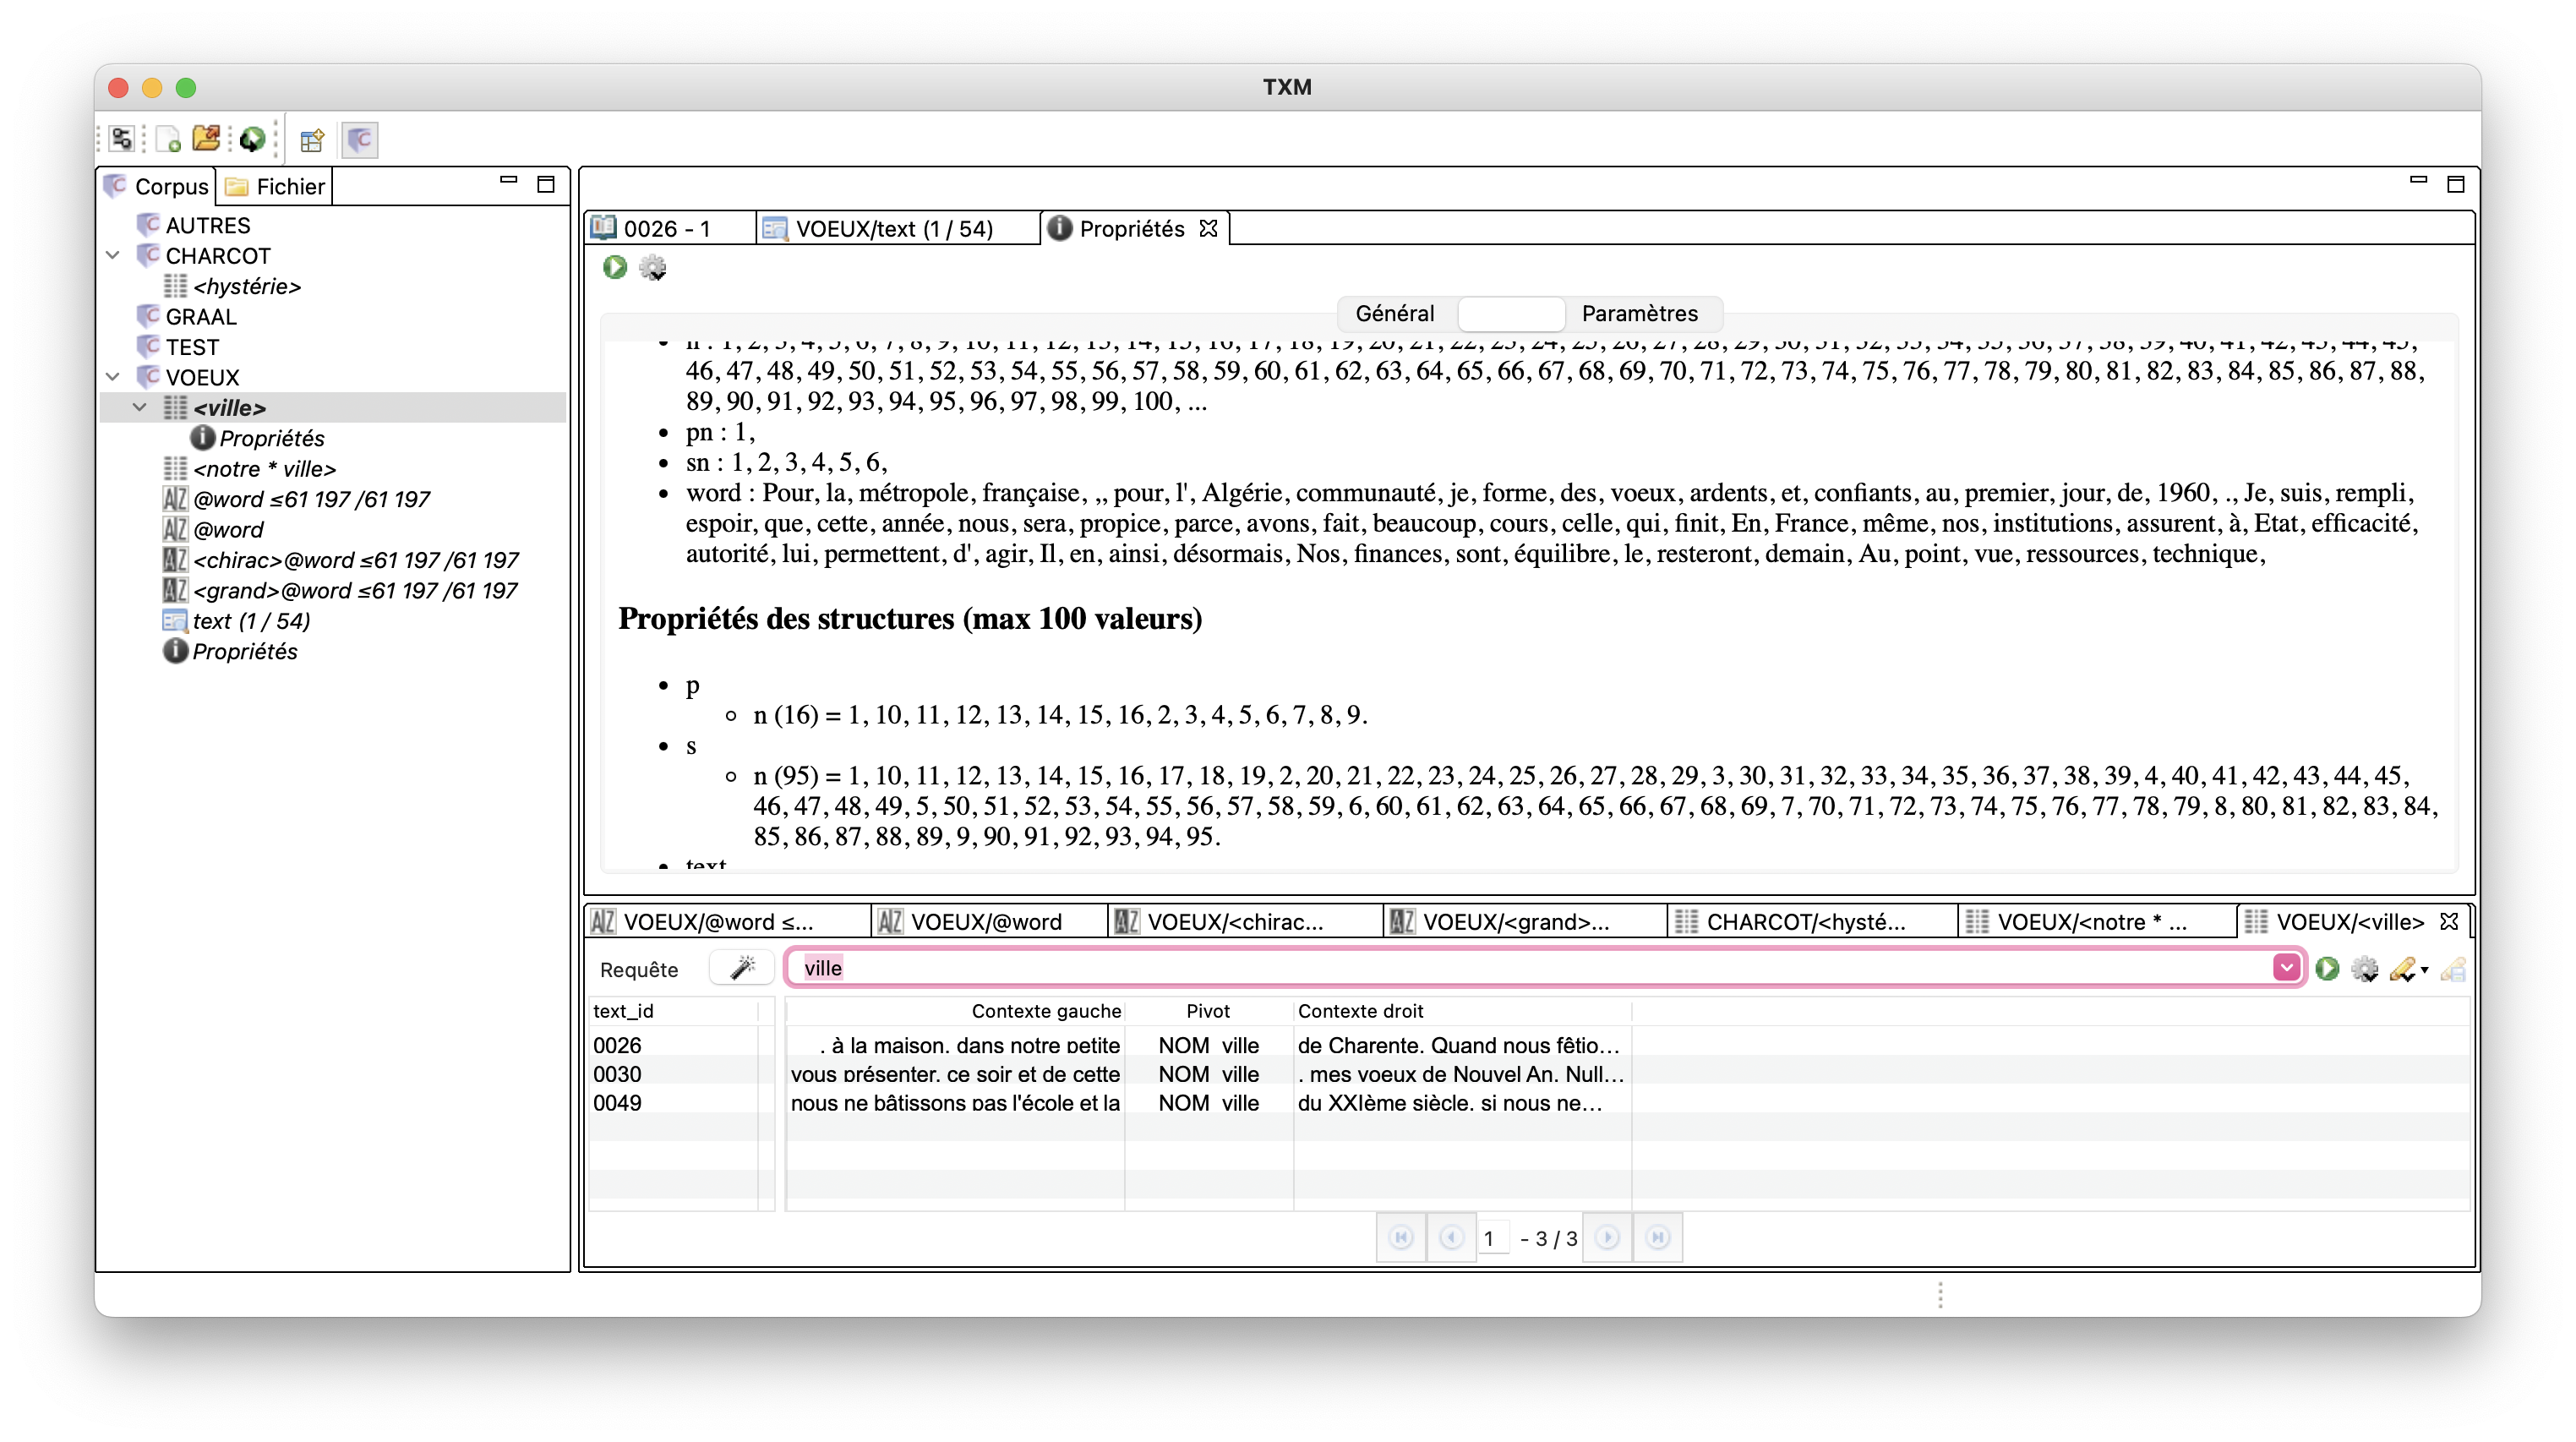
\includegraphics[width=1\linewidth]{img/affichage_proprietes_pivot.png}
		\caption{Affichages des propriétés du pivot \og{}ville\fg{} dans le corpus \texttt{VOEUX}.}
		\label{fig:ling_out_TAL}
	\end{figure}
\end{frame}

\begin{frame}{Fréquences lexicales}
	Vue des types (mots uniques) et des tokens (formes de mots)
	
	Table des fréquences : distribution par type (y compris les étiquettes \textsc{POS})
	
	Selon la loi de Zipf, on retrouve :
	\begin{itemize}
		\item en premières positions des mots grammaticaux
		\item en positions inférieures : mots sémantiquement chargés ou du genre textuel (si corpus homogène)
	\end{itemize}

	\begin{figure}[h] % Use [H] to force the figure to stay in place
		\centering
		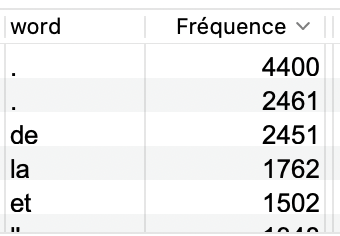
\includegraphics[width=0.25\linewidth]{img/frequences.png}
		\caption{Tableau des fréquences (extrait).}
		\label{fig:ling_out_TAL}
	\end{figure}
\end{frame}

\begin{frame}{Lexique \textit{vs.} index : deux fonctionnalités différentes}
	\bolder{Lexique}
	\begin{itemize}
		\item calcule la fréquence pour une propriété de mot donné
		\begin{itemize}
		 \item forme, lemme$\dots$ mais pas d'expressions complexes
		\end{itemize}
		\item première visualisation du corpus : thèmes, \textit{hapax}
	\end{itemize}
	\bolder{Index}
	\begin{itemize}
		\item calcule la fréquence d'une expression (mot unique ou non)
		\item agit comme un filtre sur le lexique
		\item adapté à la recherche à tâtons dans le corpus
	\end{itemize}
\end{frame}

\begin{frame}{Lexique \textit{vs.} index}
		\begin{figure}[h] % Use [H] to force the figure to stay in place
		\centering
		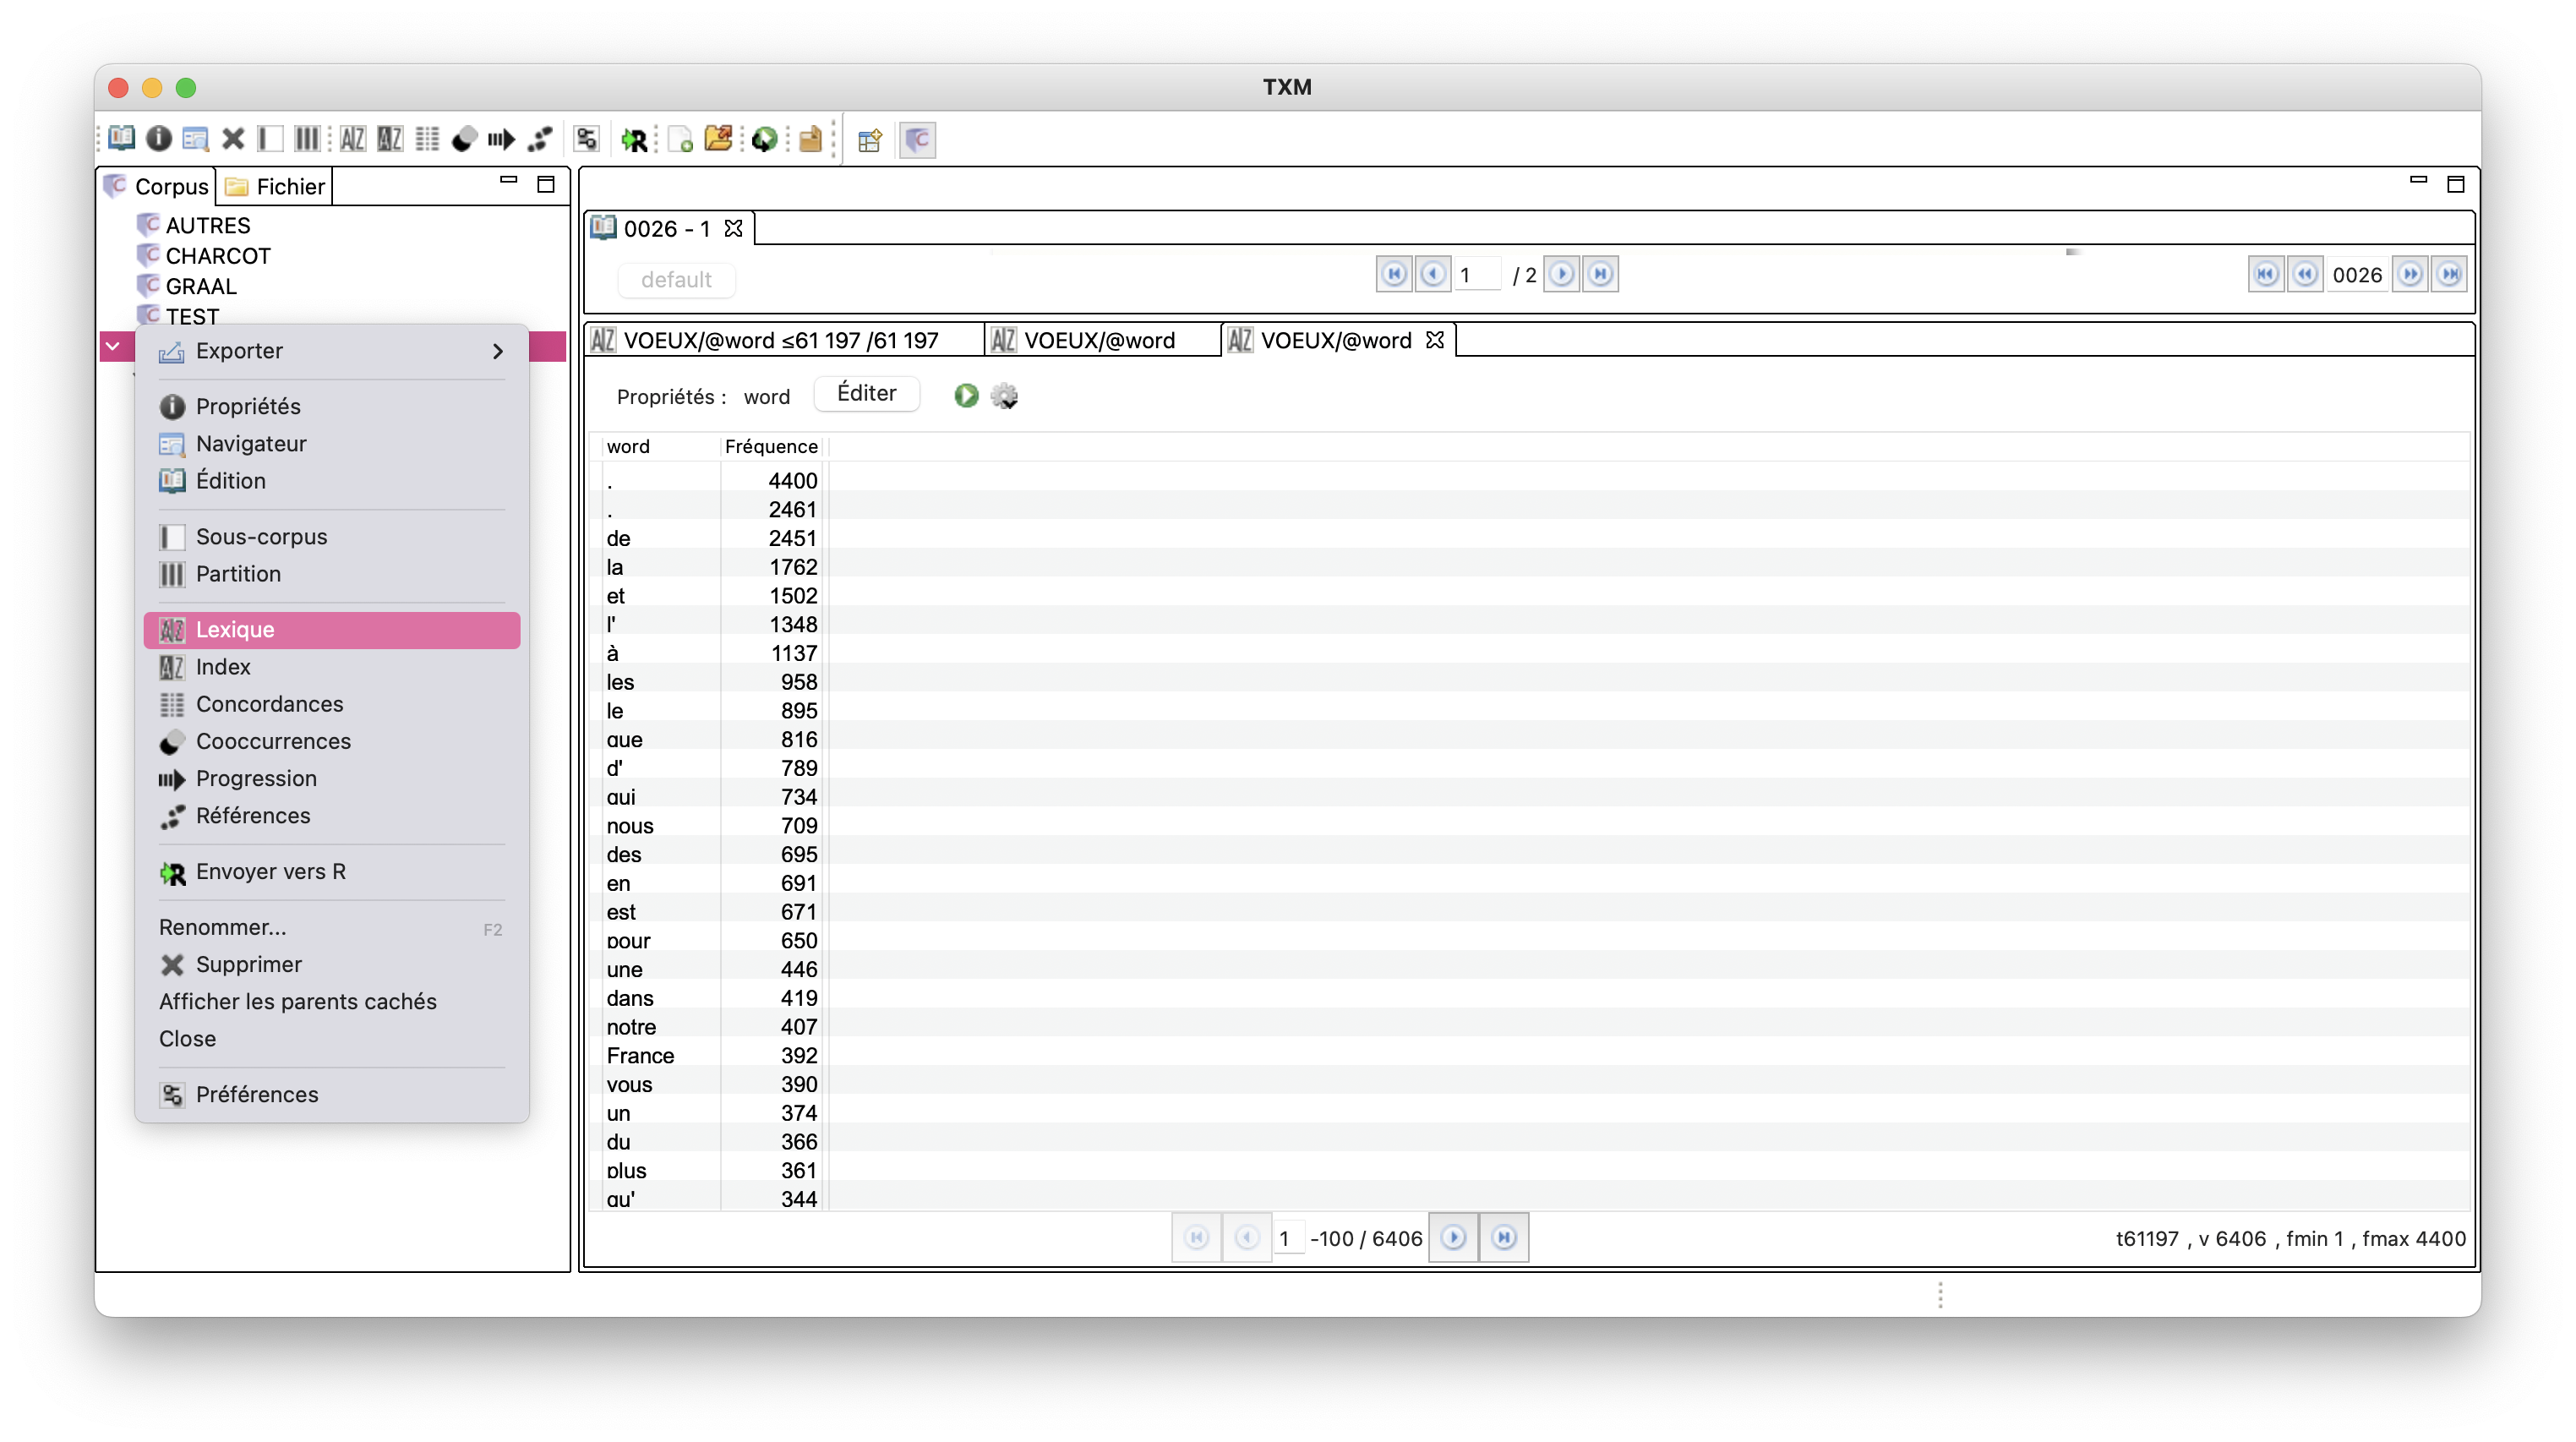
\includegraphics[width=1\linewidth]{img/lexique.png}
		\caption{Lexique (extrait).}
		\label{fig:ling_out_TAL}
	\end{figure}
\end{frame}

\begin{frame}{Lexique \textit{vs.} index}
	\begin{figure}[h] % Use [H] to force the figure to stay in place
		\centering
		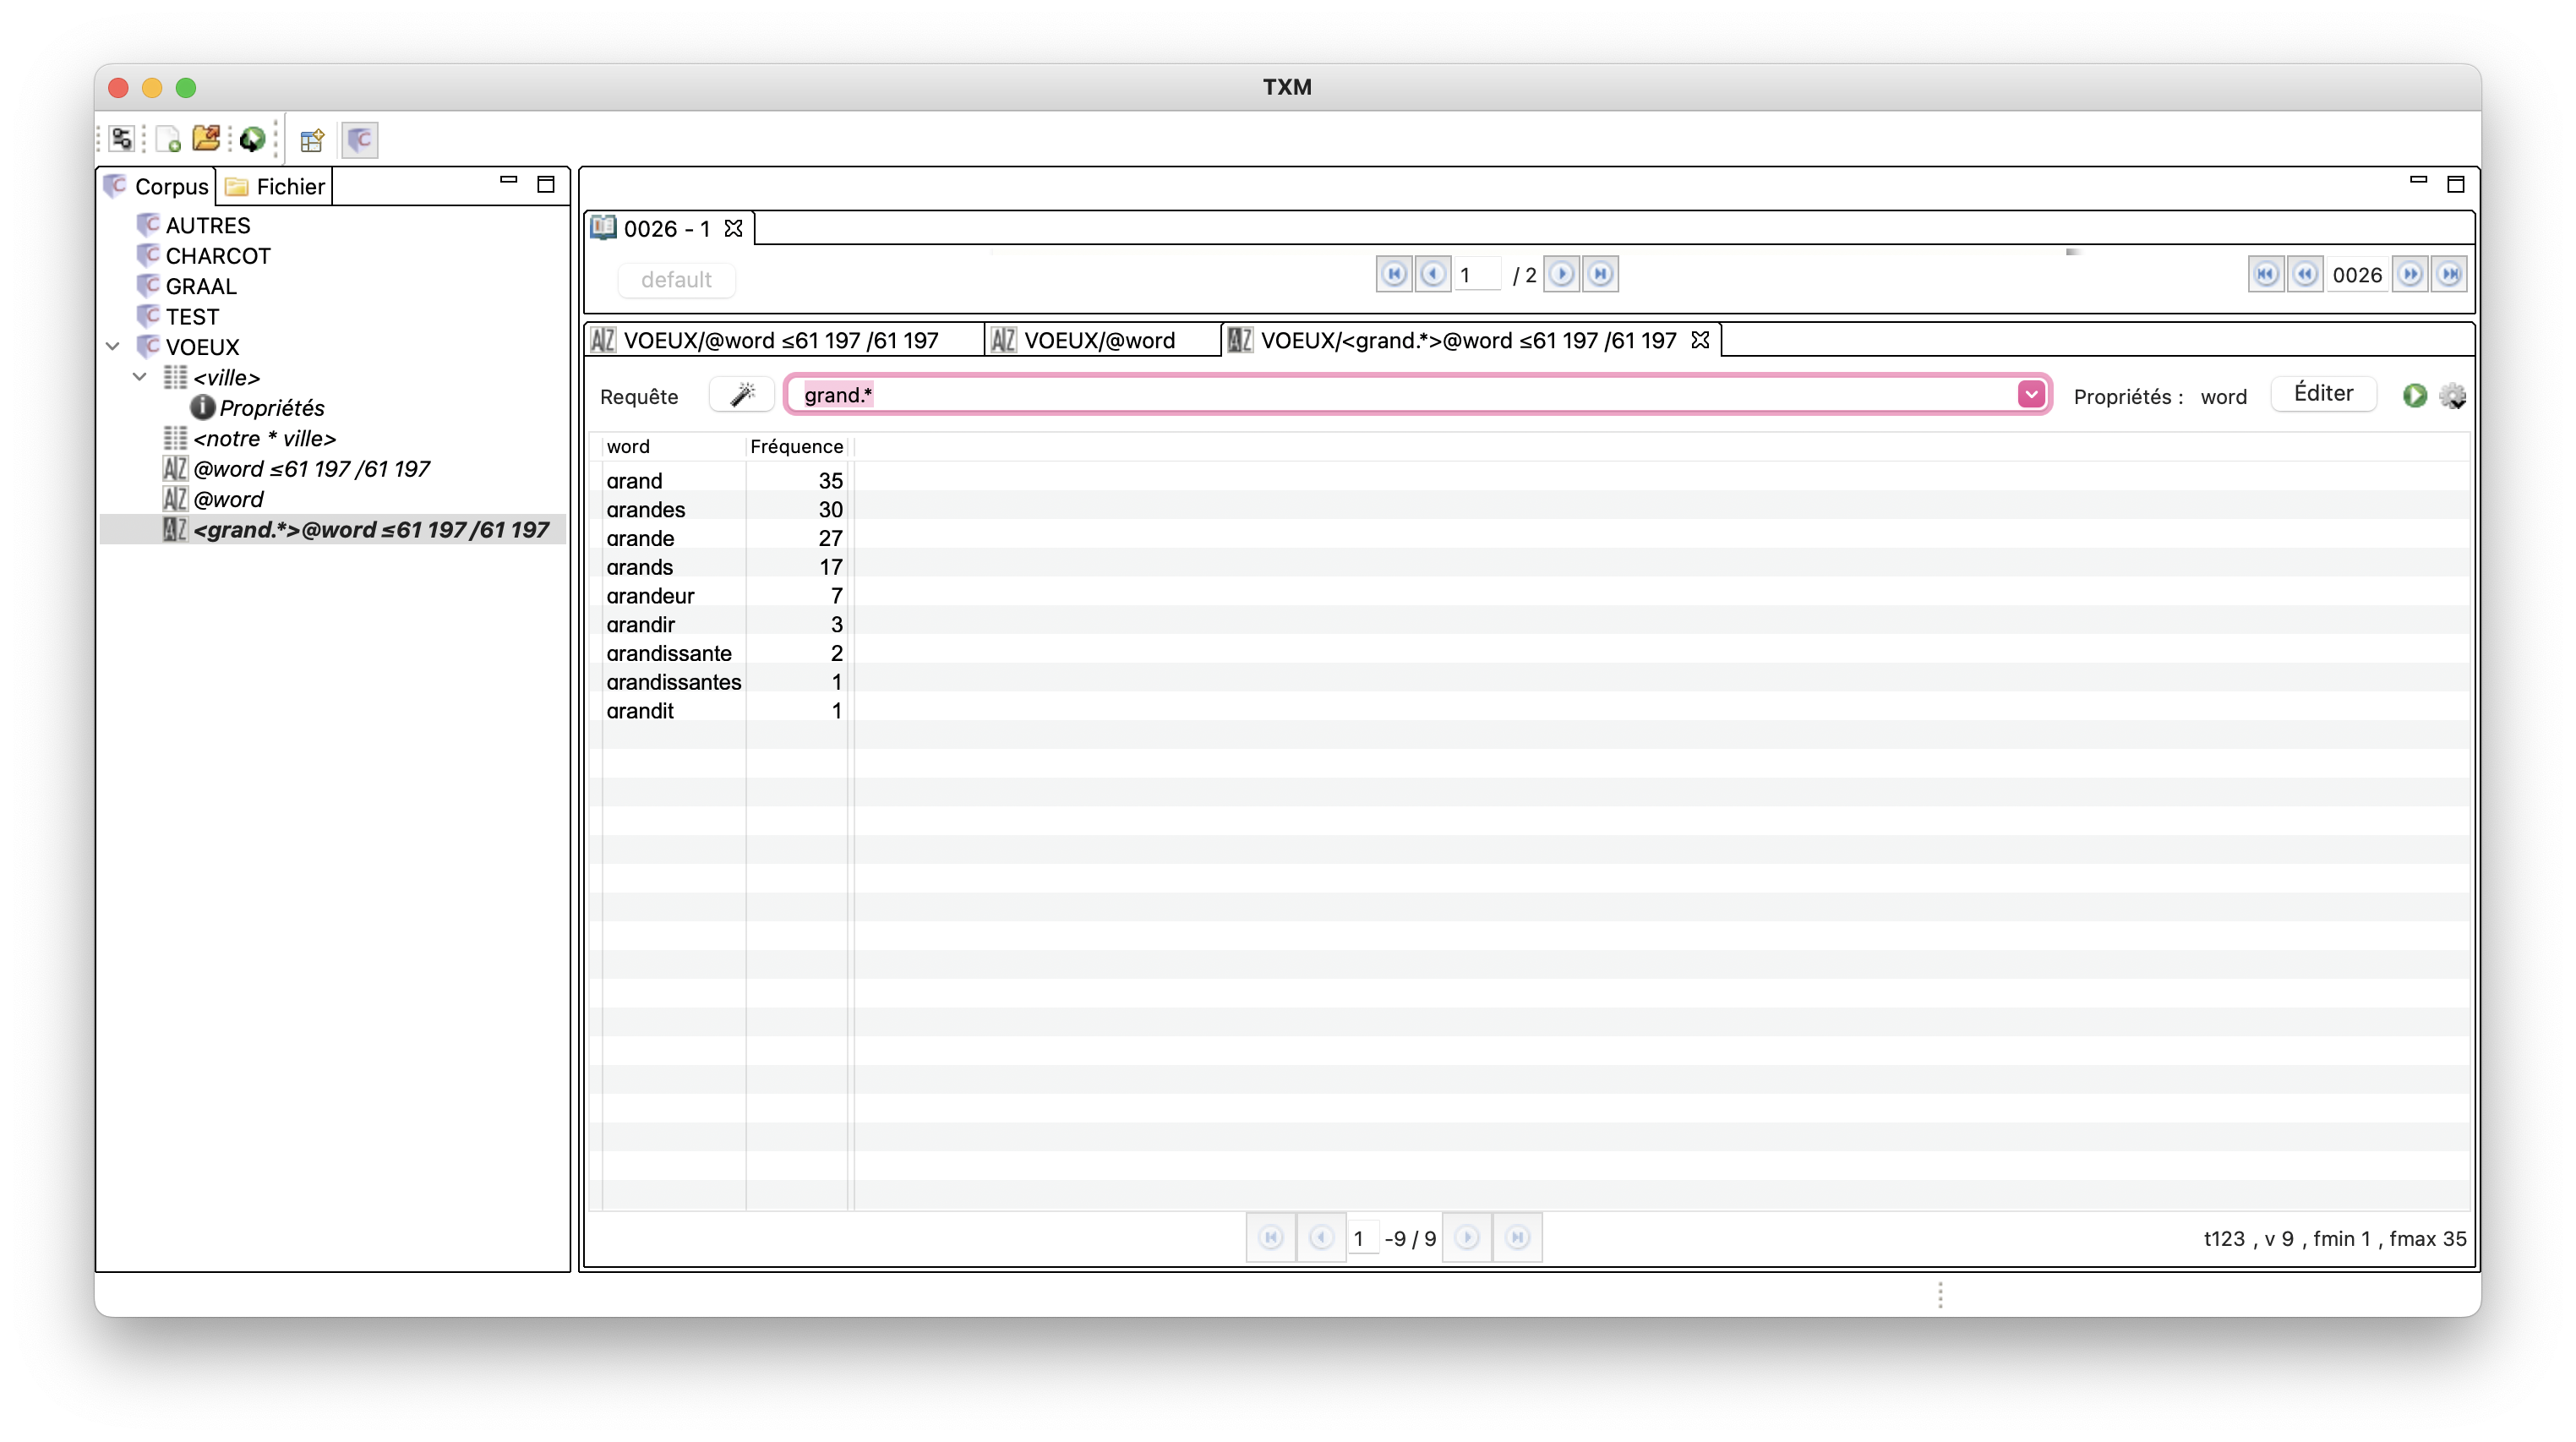
\includegraphics[width=1\linewidth]{img/index.png}
		\caption{Index (extrait).}
		\label{fig:ling_out_TAL}
	\end{figure}
\end{frame}

\begin{frame}{\textsc{CQL} -- \textit{Corpus Query Language}}
	\begin{itemize}
		\item expressions régulières : 
		\begin{itemize}
		\item \texttt{Europe|européen.∗}, \texttt{[]} (un mot)
		\item \texttt{\&} et \texttt{|} (opérateurs booléens)
		\end{itemize}
		\item neutralisations (à ajouter après l’expression) :
		\begin{itemize}
			\item \texttt{\%c} pour neutraliser la casse (\texttt{"europe"\%c})
			\item \texttt{\%d} pour neutraliser les diacritiques (accents, cédille)
			\item $\dots$
		\end{itemize}
		\item assistant de requête
		\item tri du contexte droit et du contexte gauche
	\end{itemize}
\end{frame}

\begin{frame}{Relation entre \texttt{TXM} et \textsc{TAL}}
	\texttt{TXM} n’est pas un outil de \textsc{TAL} en tant que tel, mais 
	\begin{itemize}
		\item il intègre des fonctionnalités de \textsc{TAL}, \textit{via} \texttt{TreeTagger}
		\item il permet d’explorer les corpus et de les analyser manuellement (préalable au \texttt{TAL})
	\end{itemize}
\end{frame}

\section{Bien démarrer avec \texttt{TXM}}

\begin{frame}{Installation}
	Téléchargement du logiciel + extension \texttt{TreeTagger} et prérequis :\\ \url{https://txm.gitpages.huma-num.fr/textometrie/files/software/TXM/0.8.3/}
\end{frame}

\begin{frame}[allowframebreaks]
		\printbibliography
\end{frame}


\end{document}